\documentclass[oneside,13pt,a4paper]{report}

% Chargement d'extensions
\usepackage[utf8]{inputenc}    
\usepackage[french]{babel}
\usepackage{graphicx}
\usepackage[top=2.5cm, bottom=3cm, left=3cm, right=3cm]{geometry}
 
% Informations le titre, le(s) auteur(s), la date
\title{Moteur de Requêtes SQL Simples}
\author{
    Massili KEZZOUL \and 
    Chakib ELHOUITI \and
    Ramzi ZEROUAL \and
    Belkassim BOUZIDI \and
    Fei YANG
}
\date{\today}


\begin{document}
    %\maketitle
    \begin{titlepage}
        \centering        
        {\scshape\LARGE Univérsité de Montpellier\par}
        {\scshape\Large Rapport de projet\par}
        \vspace{1.5cm}
        {\huge\bfseries Moteur de requêtes SQL simples\par}
        \vspace{2cm}
        {\Large\itshape 
            Massili KEZZOUL \\
            Chakib ELHOUITI \\
            Ramzi ZEROUAL \\
            Belkassim BOUZIDI \\
            Fei YANG \\
        \par}
        
        \vspace{1.5cm}

        {\Large\itshape 
            Encadrante :\par
            Mme. Anne-Muriel \textsc{Chifolleau}
        \par}
        
        \vspace{2cm}

        
\includegraphics[width=0.5\textwidth]{img/univ-montpellier.png}\par\vspace{1cm}

        \vfill

        % Bottom of the page
        {\large \today\par}
    \end{titlepage}

    \tableofcontents

% Espacement entre les paragraphes  
\parskip=5pt

% ------------------------------------- %
% Introduction
% ------------------------------------- %

    \chapter{Introduction}

        Dans le cadre du module de projet informatique du second semestre de L2, nous avons mis au point un moteur d’évaluation de requêtes SQL en mémoire vive.

        Les requêtes considérées seront des requêtes simples de la forme : « SELECT … FROM … WHERE … »  sans imbrication.

        À partir d’un ou plusieurs fichiers csv, Comma Separated Value, il est demandé de construire une représentation en mémoire des données et d’implémenter les procédures de projection, sélection et de jointure découlant de l’interrogation SQL.

        Il s’agit principalement de reproduire les fonctionnalités de bases d’un gestionnaire de données qui est Oracle .

        Notre groupe est composé de quatre personnes, Massili Kezzoul, Chakib Elhouiti, Ramzi Zeroual et Belkassim Bouzidi, et nous sommes encadrés par Mme Anne-Muriel Chifolleau. La réalisation du projet s’est déroulée sur une période de X semaines, de mi-janvier à avril 2019.

% ------------------------------------- %
% Organisation
% ------------------------------------- %

    \chapter{Organisation du projet}
        \section{Méthodes d’organisation}

            Afin de mener à bien le développement du projet, nous avons décidé de travailler un maximum de temps ensemble et de manière très régulière. Nous nous sommes réunis trois à quatre fois par semaine afin de faire le point sur l’avancement du projet et de définir les objectifs restant à atteindre.
            
            Enfin, selon l’état d’avancement du moteur de requêtes, nous réalisons les tâches en retard durant le week-end pour ne pas cumulé de retard et respecter l’intégralité le cahier des charges.
            
            Toutes les semaines, nous nous sommes réunis avec notre encadrante, Mme Anne-Muriel Chifolleau, afin de faire le point sur l’état du projet. Ces réunions nous on également permis de bénéficier des précieux conseils de notre encadrante.

        \section{Decoupage du projet}

            Nous avons découpé la réalisation du projet en trois grandes phases.

            \subsection{Phase de modélisation}
                
                Durant cette étape, nous nous somme réunis pour définir les fonctionnalités demandés par le projet. Notamment séparer les fonctionnalités importants de celle moins importantes. Nous avons également choisi les outils de travail collaboratif et les principales technologies utilisés, ainsi que une première modélisation du projet.

            \subsection{Phase de développement}
                
                Durant cette phase, nous avons commencer à implémenter les différentes fonctionnalités que nous avons modélisé lors de l’étape précédente, toute en améliorant la modélisation au fur et à mesure de l’avancement de notre projet. Nous avons notamment réaliser des tests pour les différents modules afin de s’assurer de leur bon fonctionnement.
            
            \subsection{Finalisation du projet}

                Cette étape a consisté en la réalisation des tests finaux afin de s’assurer que le moteur de requêtes fonctionne en toute circonstance et éventuellement corriger les bogues qui peuvent apparaître.
            
        \section{Outils de collaboration}

            Afin de s’organiser, nous avons décider d’utiliser Git au travers du serveur GitLab héberger par le service informatique de la faculté. En effet le logiciel libre Git a facilité grandement la collaboration entre nous. Le serveur GitLab quant à lui est fourni gratuitement par le service informatique la faculté.

% ------------------------------------- %
% Le langage SQL
% ------------------------------------- %

    \chapter{Le langage SQL et les bases de données}
    
        Le domaine dans le quelle ce situ notre projet est la gestion d’une base de donnée en utilisant le langage SQL . 

        \section{Qu’est-ce qu’une donnée}

            En termes simples, les données peuvent êtres des faits liés a tout objet considéré .
            Par exemple, un nom, un age, une taille, un poids ect. Sont des données.

        \section{Présentation d’une base de donnée}

            Une base de données regroupe et stock un ensemble d’informations organisées et accessibles qui peuvent être modifiées et mises à jour. En informatique une base de données est la pièce centrale d’un système d’informations ou d’un système de base de donnée , qui régit la collecte, le stockage , le retraitement et l’utilisation de données . Ce dispositif comporte souvent un logiciel moteur dont notre projet.

        \section{Un système de gestion de base de données}

            Le système de gestion de base de données (SGBD) est un ensemble de programmes qui permet à ses utilisateurs d'accéder à une base de données, de manipuler des données, de générer des rapports / de représenter des données.
            Cela permet également de contrôler l'accès à la base de données.

        \section{Le langage SQl}

            Le langage de requête structuré (SQL) prononcé comme "S-Q-L" est en fait le langage standard pour traiter les bases de données relationnelles.

            La programmation SQL peut être utilisée efficacement pour insérer, rechercher, mettre à jour et supprimer des enregistrements de base de données.

            En fait, il peut faire beaucoup de choses, y compris mais sans s'y limiter, l'optimisation et la maintenance des bases de données.

            Les bases de données relationnelles telles que la base de données MySQL, Oracle, le serveur Ms SQL, Sybase, etc. utilisent SQL! Comment utiliser les syntaxes SQL?

            Les syntaxes SQL utilisées dans ces bases de données sont presque similaires.

            Example de requête SQL : \nomprog{SELECT * FROM Members WHERE Age > 30;}
% ------------------------------------- %
% Présentation du projet : moteur de requêtes SQL simples
% ------------------------------------- %

    \chapter{Présentation du projet : moteur de requêtes SQL simples}

    \section{Présentation générale}

        Notre projet consiste à concevoir et implémenter un moteur de requêtes SQL simples , nous avons donc à partir d’un ou plusieurs fichiers csv donnés permettre d’exécuter une requête SQL simple .

        Il s’agit  donc de crée une passerelle entre la personne qui exécute la requête SQL et le fichier csv qui contient les informations nécessaire afin réaliser cette requête SQL , notre programme doit analyser une requête et la décompose en 3 : « SELECT... » « FROM ... » « WHERE ... » et qui en fonction de linges de code spécifique à ces 3 méthodes réanalyser ces 3 parties pour savoir quelle attributs sélectionner , comment combiner différents tableaux , comment trier le résultat etc … 

        L’analyse syntaxique n’est qu’une petite partie de la tâche , après avoir décomposé la requête en clauses et expressions logique , il faut ‘traduire’ les noms des tableaux et les atributs et y avoir accès pour lire les données des fichiers csv donné . Il faut appliquer des méthodes aux données pour déterminer quelles lignes inclure et lesquelles filtrer. Il est nécessaire de joindre des lignes de plusieurs fichiers de données en les mettant en correspondance selon les expressions de requêtes SQL. Il faut extraire des sous-ensembles de champs de chaque ligne . 
        
        Un moteur de requêtes SQL simples est un logiciel qui :
        \begin{itemize}
            \item Reconnaît et interprète le langage SQL 
            \item Implémente l’accès aux données en lecture.
        \end{itemize}

    \section{Les Fonctions Principales}

        \subsection{La sélection}

            La sélection est la ou les conditions finales afin d'effectuer la requête SQL , comme le but d'une requête SQL est d'extraire des informations spécifique dans des bases de données , la sélection permet de spécifier la requête plus en profondeur c.à.d de sélectionner seulement les éléments du ou des tableaux qui répondent a certain critères donné par la personne qui exécute la requête et de faire la concaténation de ces éléments là .

    	    Nous séparons chaque condition de sélection avec des opérateurs logiques (noté : \nomprog{AND} et \nomprog{OR}) .

	        La condition en elle même est composé de 3 parties (noté : A * B) où A et B sont les opérandes et * l'opérateur , ces conditions sont des comparaisons entre A et B , ces comparaisons sont de base de type "CHAR" mais peuvent être de "INT" ou "DATE" en fonction de la condition en elle même.

        \subsection{La projection}

        \subsection{La jointure}

            La jointure est un produit cartésien entre un ou plusieurs tableaux donnés par la personne qui effectue la requête puis d'une sélection , les tableaux donnés sont séparé par des virgules lors de initialisation de la requête .
	        
            Le produit cartésien entre un tableau A et B et un tableau composé de l'ensemble des couples possible entre leurs éléments respectives, ainsi nous aurons en résultat un tableau A*B.

            -Dans notre programme nous exécutons la projection et la sélection sur le tableau finale. -

	        Le produit cartésien est donc la base et la première tache qu’effectue notre programme lors de l’exécution. Un exemple est plus parlant qu'une longue explication , prenons deux tableaux N et B nous effectuons un PC entre ces deux tableaux N*B, le résultat de l’exécution de la jointure donnera un nouveau tableau ((N*B) - Sélection).

% ------------------------------------- %
% Conception du Moteur de Requêtes
% ------------------------------------- %

    \chapter{Conception du Moteur de Requêtes}

        \section{Structure de données}
            Avant toute chose, il faut commencer par charger les données en mémoire. Pour cela il faut commencer par savoir comment stocker efficacement les données pour pouvoir effectuer dessus les traitements demandés par l’utilisateur.

            Pour cela nous avons donc réaliser un diagramme UML schématisant les classes utilisé pour stocker en mémoire l’ensemble des données utilisé pour la requête.

            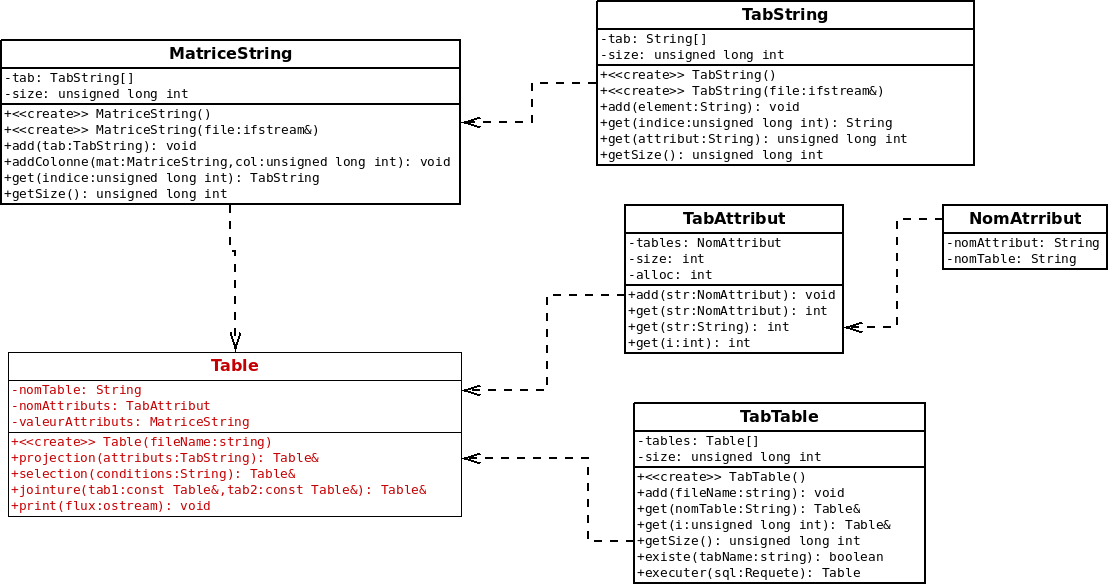
\includegraphics[width=0.5\textwidth]{img/sql.png}\par

        \section{Traitement des données}

            \subsection{La sélection}

            \subsection{La projection}

            \subsection{La jointure}

% ------------------------------------- %
% Implementation
% ------------------------------------- %

    \chapter{Implementation}

        \section{Choix de la téchnologie}

        \section{Développement}

            \subsection{Chargement des données}

            \subsection{restitution des données (affichage)}

            \subsection{Selection ...}

        \section{Logiciel : terminal / ligne de commande / formt des données en entrée et sortie}

        \section{Test}


% ------------------------------------- %
% Bilan et difficultés rencontrées
% ------------------------------------- %

    \chapter{Bilan et difficultés rencontrées}

% ------------------------------------- %
% Perspective
% ------------------------------------- %

    \chapter{Perspective}

% ------------------------------------- %
% Annexes
% ------------------------------------- %

    \chapter{Annexes}

    
\end{document}